\chapter{Проектирование архитектуры плагина} \label{ch2}
	
% не рекомендуется использовать отдельную section <<введение>> после лета 2020 года
%\section{Введение} \label{ch2:intro}
В данной главе будет проведено проектирование разрабатываемого плагина: будет описана архитектура построения плагинов в Jenkins, а также архитектура разработки, будут выбраны инструменты разработки, а также рассмотрена функциональная модель системы. Поскольку плагин разрабатывается для системы Jenkins, то отладку и тестирование будем проводить в этой системе.

\section{Модель системы} \label{ch1:sec1}

Диаграмма вариантов использования, показывающая функционал плагина отображена на рис.2.1. На данной диаграмме основное внимание также уделяется процессу визуализации статистики метрик сборок. Основное действующее лицо одно - это пользователь системы, который запускает сборки и работает в CI системе, это может быть любой участник команды, который задействован в разработке, тестировании, доставке и внедрению приложения. В данном случае все эти роли представлены на диаграмме как разработчик.

\begin{figure}[ht!] 
	\center
	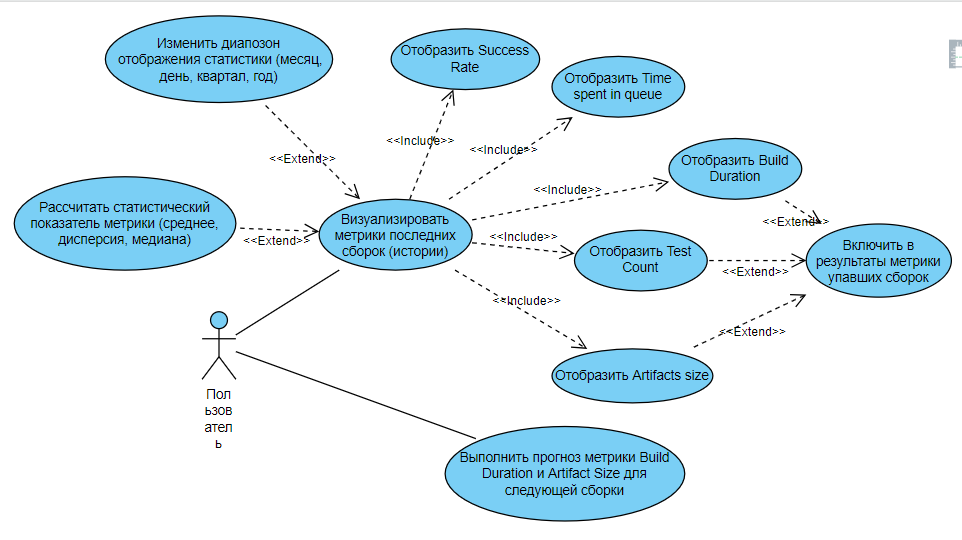
\includegraphics [scale=0.7] {my_folder/images//usecase3}
	\caption{Use case } 
	\label{fig:usecase3}  
\end{figure}

Функциональная модель в нотации IDEF0 отображена на рис.2.2. Декомпозиция процесса отображена в приложении П5.1-2 Основное внимание на диаграмме уделяется визуализации статистики сборок, поскольку это изначально является целью разработки. Также там будут отражены дополнительные функции такие как фильтрация, и высчитывание статистик метрик.

\begin{figure}[ht!] 
	\center
	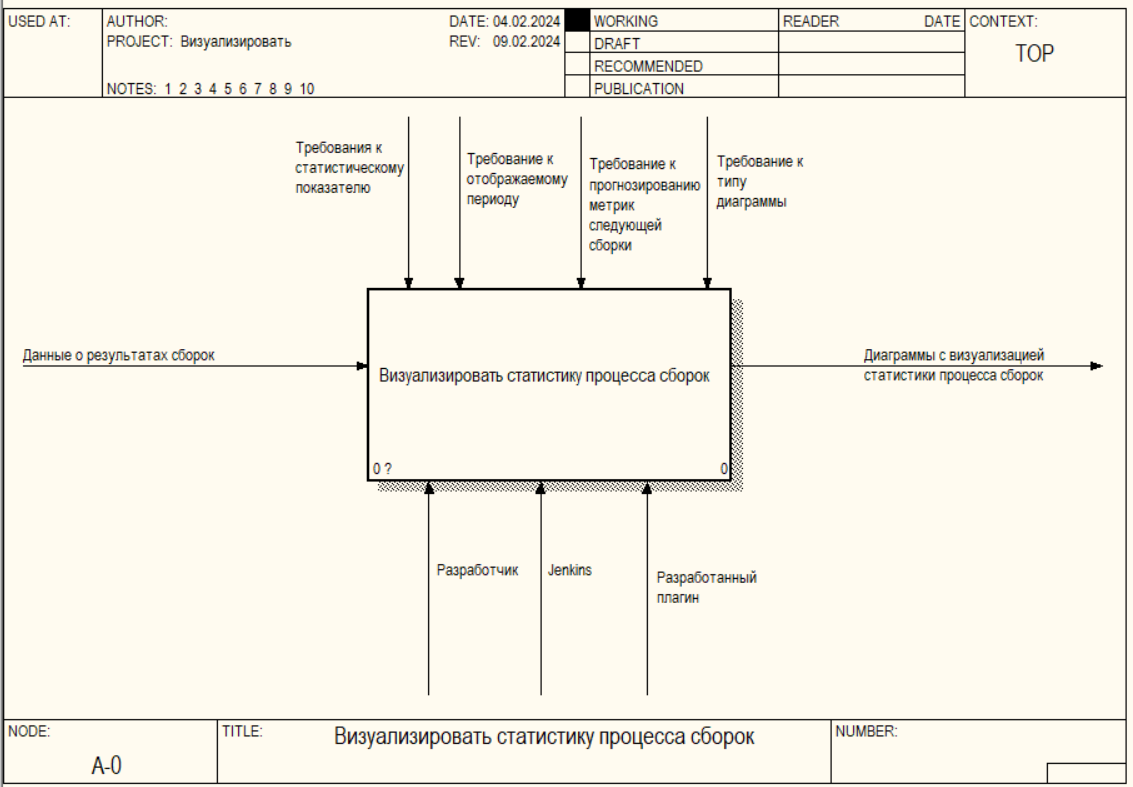
\includegraphics [scale=0.7] {my_folder/images//ide1_2}
	\caption{Процесс визуализации сборок} 
	\label{fig:er1}  
\end{figure}

\section{Архитектура Jenkins} \label{ch1:sec2}

Перед объяснением построения архитектуры плагинов Jenkins, необходимо привести схему архитектуры Jenkins, где будет отображено место разрабатываемых плагинов в CI системе. Архитектура Jenkins представлена на рис.2.3. Установленные плагины Jenkins-CI, а также локальные сценарии и приложения выполняются на сервере Jenkins-CI и предоставляют расширяемый набор функций управления и обработки данных \cite{article}.

\begin{figure}[ht!] 
	\center
	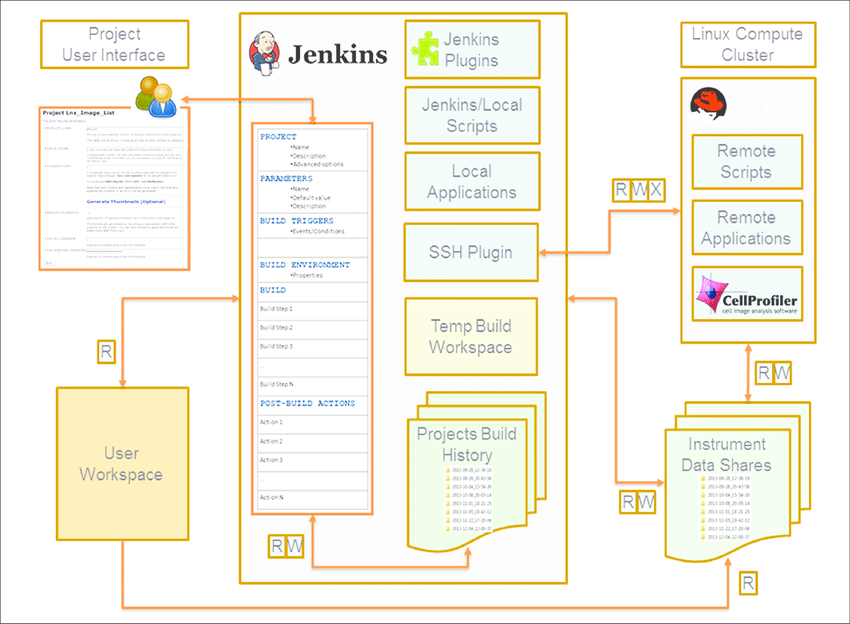
\includegraphics [scale=0.47] {my_folder/images//ArchitectureJenkins}
	\caption{Архитектура Jenkins \cite{article}} 
	\label{fig:ArchitectureJenkins}  
\end{figure}


Архитектура плагинов использует точки расширения, которые, предоставляют разработчикам плагинов возможности реализации для расширения функциональности системы Jenkins \cite{atchplugin}. Точки расширения автоматически обнаруживаются Jenkins во время загрузки системы.

В разрабатываемом плагине реализация будет происходить через класс Action. Actions являются основным строительным блоком расширяемости в Jenkins: их можно прикреплять ко многим объектам модели, хранить вместе с ними и при необходимости добавлять в их пользовательский интерфейс.

Помимо класса Action для того чтобы создать временные действия, которые будут прикреплены к заданию Jenkins будет использован класс TransientActionFactory, который позволяет создавать действия, которые будут отображаться на страницах Jenkins только при наличии соответствующего объекта - задания.

Разработка будет выполняться в объектно-ориентированной парадигме, т.е. приложение будет разбито на классы, будет применяться наследование, полиморфизм и инкапсуляция. Все классы, которые будут разработаны для плагина отображены на рис.2.4. 

\begin{figure}[ht!] 
	\center
	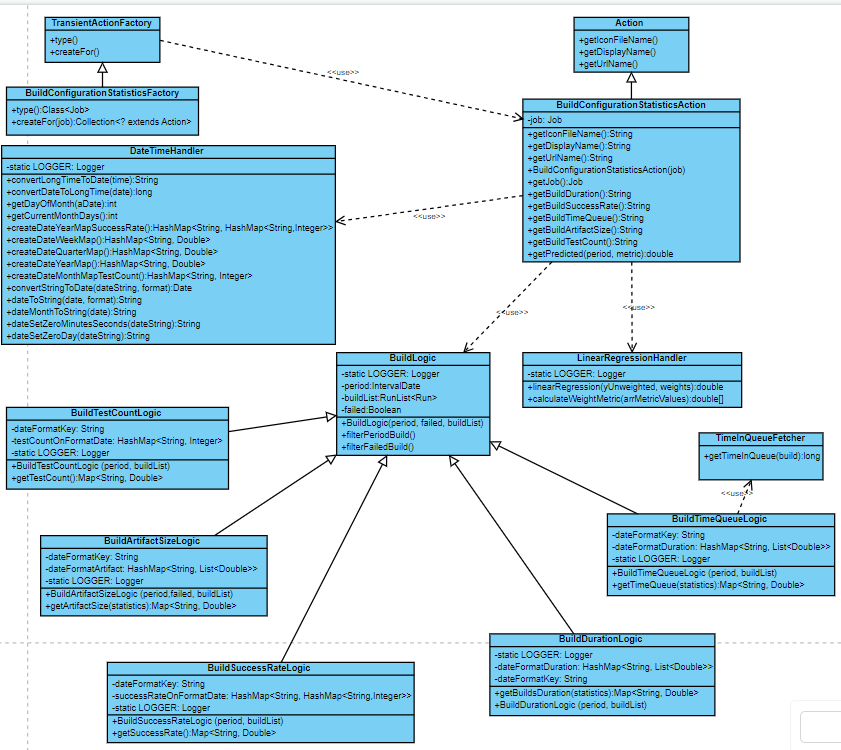
\includegraphics [scale=1] {my_folder/images//class3}
	\caption{Диаграмма классов плагина} 
	\label{fig:class3}  
\end{figure}

При рассмотрении диаграммы необходимо отметить, что два класса являются встроенными в Jenkins, это TransientActionFactory, который позволяет добавлять действия к любому типу объекта, а также интерфейс Action - добавленный к объекту модели, создает дополнительное подпространство URL-адресов под родительским объектом модели, через которое он может взаимодействовать с пользователями. Actions также способны открывать доступ к левому меню в интерфейсы Jenkins, по которому обычно производится навигация при конфигурировании сборки.

Для удобства использования плагина, предполагается добавить дополнительную ссылку в меню слева, для перехода на страницу визуализации метрик, а также динамически обновлять страницу при изменении параметров и фильтров, что и обосновывает использование данных встроенных классов.

Основная часть остальных классов требуется для работы с определенной метрикой статистики выполнения сборок Jenkins, что следует из их названия. Также будет разработан дополнительный класс DateTimeHandler, который позволит создать методы для удобной работы с датой и временем, что необходимо поскольку будет производиться преобразования одних типов дат к другим, сравнение дат между собой, а также получение определенных частей дат.

\section{Архитектура плагина} \label{ch1:sec3}

Для того чтобы визуализировать и обработать данные о сборках, необходимо получить эти данные. Для этого необходимо использовать различные методы и классы Jenkins, такие как Job - для работы с проектом (статическая сущность), а также Run для работы со сборкой (конкретные запуски Job, со временем выполнения и результатом). Внутри методов этих сущностей при их вызове будет отправляться API запрос на сервер Jenkins, который будет возвращать данные из хранилища xml файлов для каждой конкретной сборки.

После получения данных в плагине, идет их обработка и подготовка структур данных для визуализации. Вызов методов обработки данных о сборках будут происходить из Jelly файлов, в которых с помощью специальных тегов будет производиться связывание между объектами бизнес-логики Java и JS файлами, где будут создаваться графики визуализации.

Jelly для получения данных из Java использует AJAX запросы, а затем полученные данные сохраняет в DOM структуре страницы плагина. Затем с помощью JS происходит получение данных о сборках из DOM структуры и отправка в методы построения графиков.

Все взаимодействие между Java, Jelly и JS происходит с помощью JSON структур, такое решение было принято ввиду удобства работы со структурой с помощью этих инструментов. На рис.2.5 представлено изображение архитектуры плагина.

\begin{figure}[ht!] 
	\center
	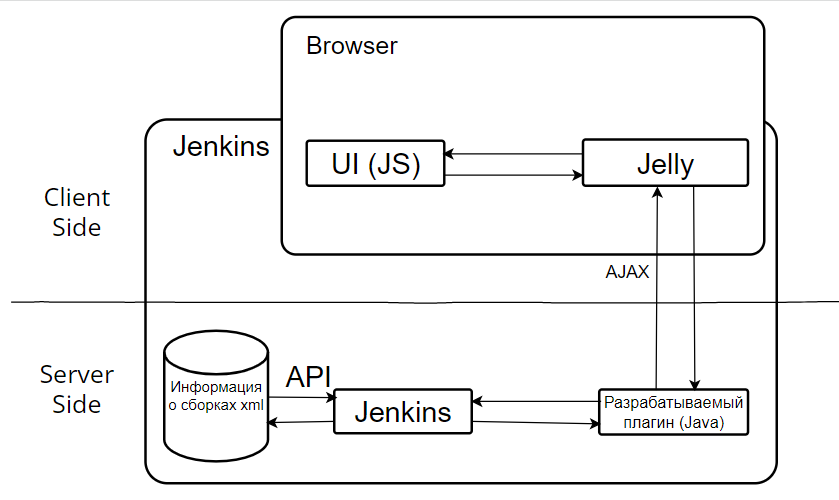
\includegraphics [scale=0.67] {my_folder/images//archpl3}
	\caption{Архитектура плагина} 
	\label{fig:ArchitecturePlugin}  
\end{figure}


\section{Языки программирования} \label{ch1:sec4}

Для программирования плагина будет использоваться язык Java. Поскольку Jenkins написан на Java, то все плагины необходимо писать на том же языке. Это является главным минусом, а возможно и сложностью при разработке плагинов на Jenkins, поскольку ограничивает свободу разработчика.

Есть возможность разработки плагина с использованием языка программирования Groovy. Groovy это динамический язык с возможностями статической типизации и статической компиляции для платформы Java \cite{groovy}, нацеленный на повышение производительности разработчиков, который плавно интегрируется с любой программой Java.

Недостатком такого выбора является то, что абсолютное большинство плагинов написано на чисто Java, а значит сообщества и поддержка при разработке на Java будет значительно большей. Также в сравнении с Groovy, Java обладает большей производительностью \cite{groovyvsjava}, статической типизацией и подходит для разработки приложений в парадигме ООП.

Java — это язык высокого уровня, который можно охарактеризовать следующими словами: объектно-ориентированный, многопоточный, динамический, высокопроизводительный и безопасный \cite{java}. Java используется для разработки высоконагруженных информационных систем, мобильных приложений, плагинов, десктопного ПО и др. К преимуществам Java также можно отнести компилируемость, что обеспечивает высокое быстродействие.

Java будет использоваться для программирования ядра плагина и бизнес-логики. Также для программирования графических компонентов, графиков и диаграмм будет использоваться язык программирования JavaScript. JS - это легковесный, интерпретируемый или JIT-компилируемый, объектно-ориентированный язык \cite{js}, основное предназначение которого выполнять сценарии на веб-страницах, что необходимо при разработке плагина, результаты которого отображаются на веб-страницах.

Помимо прочего, для стилизации компонентов веб-интерфейса будет использоваться язык каскадных таблиц стилей CSS \cite{css}, который позволит настроить удобное отображение и позиционирование элементов на странице плагина Jenkins. 

Верстка страниц будет осуществляться с помощью инструмента Jelly - все разрабатываемые плагины используют данный инструмент в Jenkins, поскольку с ним можно легко интегрировать Java, XML и JS. Jelly — это средство для преобразования XML в исполняемый код, это механизм сценариев и обработки на основе Java и XML \cite{jelly}. В Jelly можно вызывать функции Java, использовать такие синтаксические конструкции, как циклы, условия и переменные, также он позволяет легко обратиться к объектам в Java.

\section{Инструменты сборки} \label{ch1:sec5}

В качестве инструмента сборки проекта был выбран Maven, который можно использовать для создания и управления любым проектом на основе Java. Преимущества Maven были описаны в первой главе при рассмотрении инструментов сборок приложения.

Абсолютное большинство разработанных плагинов для Jenkins использует Maven, поскольку Maven предоставляет удобные архетипы для начала разработки плагинов, что делает использование того же Gradle не рациональным.


\section{Библиотеки} \label{ch1:sec6}

\subsection{Chart.js}

Поскольку проект предполагает использование графиков и диаграмм, то необходимо было выбрать инструмент для работы с графиками в Jenkins и Java, который позволит отображать графики прямо на странице задания Jenkins. В качестве этого инструмента была выбрана библиотека Chart.js, которая на данный момент является самой популярной JavaScript библиотекой по оценкам GitHub и загрузок npm \cite{chartjs}. К преимуществам данной библиотеки можно отнести: 
\begin{itemize}
	\item у Chart.js очень подробная документация;
	\item отрисовка canvas делает Chart.js очень производительным, особенно для больших наборов данных и сложных визуализаций;
	\item строит отзывчивый интерфейс - перерисовывает диаграммы при изменении размера окна для идеальной детализации масштаба.
\end{itemize}

\subsection{Gson}

Для удобства разработки и взаимодействия клиентской части с серверной необходимо, чтобы обработанные данные из Jenkins в браузер передавались в формате JSON. Для обеспечения преобразования объектов и структур Java в JSON была использована библиотека Gson от компании google. К важным особенностям и преимуществам данной библиотеки можно отнести:

\begin{itemize}
	\item легкость в использовании;
	\item отсутствие требования размещения аннотаций Java в пользовательских классах \cite{gson};
	\item поддержка Java Generics.
\end{itemize}

\subsection{Apache Commons Math}

Поскольку одним из требований к плагину является работа с математической статистикой для обработки метрик сборок, а также прогнозирование значений метрик, то необходима библиотека, которая реализует данный функционал. В качестве такой библиотеки была выбрана Apache Commons Math. Commons Math это библиотека легких, автономных математических и статистических компонентов, решающая наиболее распространенные проблемы \cite{commath}, связанные со статистикой. Преимущества использования библиотеки:

\begin{itemize}
	\item скорость математических вычислений выше, чем у стандартных средств Java;
	\item открытый исходный код;
	\item функции для статистической обработки и анализа данных (линейная регрессия).
\end{itemize}

\subsection{Junit}

Для того чтобы, протестировать разработанный плагин, будут написаны unit тесты. Поскольку разработка плагина будет вестись на языке Java, то для написания тестов будет использована Java инструмент. В качестве такого инструмента был выбран Junit, который состоит из следующих компонентов:  JUnit Platform, JUnit Jupiter, JUnit Vintage \cite{junit}. Основными преимуществами инструмента являются:

\begin{itemize}
	\item популярность и большое сообщество;
	\item использование для написания тестов Java (без дополнительных фреймворков и языков);
	\item совместимость с Java инструментами (Maven, Gradle).
\end{itemize}

\subsection{Mockito}

Поскольку функционал плагина использует обращение к структурам Jenkins (Job, Run), для тестирования необходимо использовать заглушки этих структур. Для работы с заглушками была выбрана библиотека mockito, которая была выбрана из-за следующих особенностей, причин и преимуществ:

\begin{itemize}
	\item сообщество StackOverflow назвало Mockito лучшим фреймворком для заглушек на Java \cite{mockito};
	\item входит в число 10 лучших библиотек Java среди всех библиотек;
	\item позволяет писать читабельные тесты, использовать BDD подход.
\end{itemize}

\section{Выводы} \label{ch1:sec7}

В данной главе было проведено проектирование плагина, составлена use-case диаграмма и диаграмма классов, построена функциональная модель системы, описана архитектура Jenkins, а также описана архитектура, разрабатываемого плагина. Затем были выбраны инструменты разработки плагина.


%% Вспомогательные команды - Additional commands
%
%\newpage % принудительное начало с новой страницы, использовать только в конце раздела
%\clearpage % осуществляется пакетом <<placeins>> в пределах секций
%\newpage\leavevmode\thispagestyle{empty}\newpage % 100 % начало новой страницы